\section{Project Stage}
\subsection{System Architecture}

\begin{figure}[H]
	\centering
	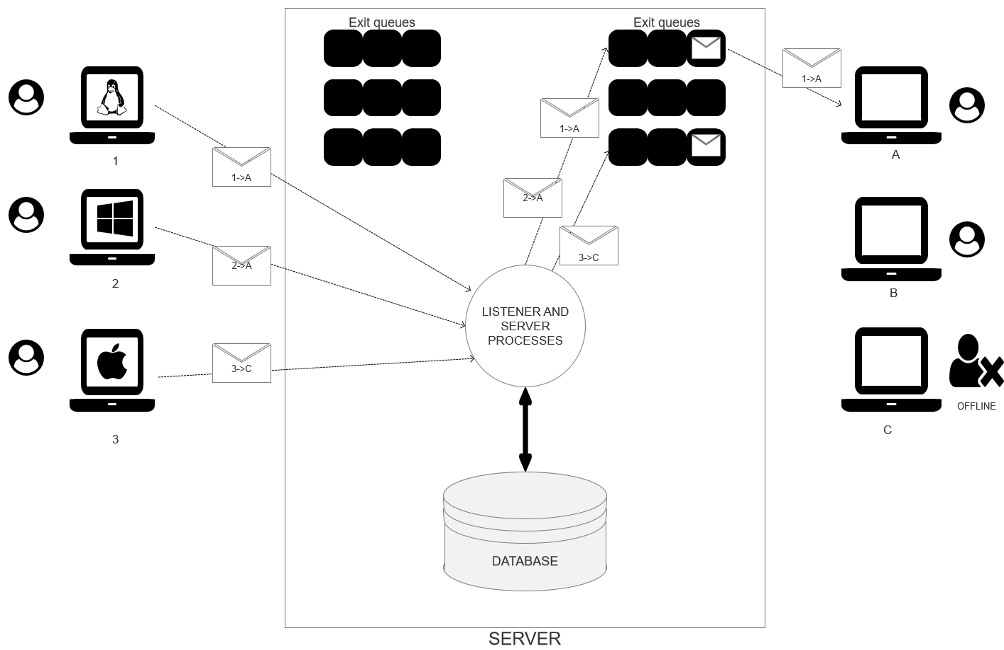
\includegraphics[width=\textwidth]{img/systemArchitecture.png}  
\end{figure}

As shown in the previous picture, the application is based on a client-server architecture, in which each client, in order to send a \textbf{message} to a \textbf{user}, contacts the main server which is in charge of determining receiver’s physical address and forward the \textbf{message} if it is online.
In the image some typical scenarios are represented to help better understand how \textit{Unisup} works. In particular:
\begin{enumerate}
	\item The message 1 $\xrightarrow{}$ A is sent from the client 1 destined to the client A:  it arrives at the main server that pushes it into the corresponding queue. The client A is online and there is no message to consume on the queue, so it is immediately forwarded.
	\item The message 2 $\xrightarrow{}$ A is sent from the client 2 destined to the client A:  as the previous one, it is pushed into A’s queue but this time the channel is busy. The message will be forwarded as soon as the channel comes idle again.
	\item The message 3 $\xrightarrow{}$ C is sent from client 3 destined to C: again, it is pushed on the correct queue. C is offline, so the message is not forwarded; it will be delivered as soon as C turns online again.
\end{enumerate}	
The OS picture inside clients means that the system works on every OS.
Eventually, the database icon has been added since it is required for mapping clients’ addresses and store chat histories. 


\subsection{Clients}
\subsubsection{Role of the Client}
The \textbf{client} is the principal actor of our application.
As described in the use cases analysis the  \textbf{client} i can register to the application, sign in into his/her account, then he/she can do all the operation of a typical instant-message application. So the  \textbf{client} i can send/receive messages and read old messages through clicking on chats. 
Because the applicative isn’t bound to a specific client, as \textit{Whatsapp} is, multiple users can use the application simply accessing to their account.

\subsubsection{Technologies}
The applicative code runs entirely on the clients: every interaction with the GUI is handled locally and may trigger a send request to the server. The principles technologies used in the client side are JavaFX and Jinterface.
\begin{itemize}
	\item The GUI is implemented using JavaFX classes, some of them were extended for creating ad-hoc classes that can be found in the javafxexstension package. The use of JavaFX is due to make the application more user-friendly.
	\item The Jinterface package provides a set of tools for communication with Erlang processes. In this way the client can send messages to the server.
\end{itemize}

\subsection{The Server}
\subsubsection{Role of the Server}
The server is the core of our system, every client have to communicate with it if they what to procede with any of the operation listed in chapter 2.1.

\subsubsection{Implementation of the Server}
The server is completely written in Erlang. 
Mirco add something about the listener and the gen\_server!

\subsubsection{Persistent Data Storing}
For storing all the information regarding the users and their relative messages we make use of Mnesia. The choice to use Mnesia is driven by the fact that Mnesia is designed with requirements like the following:
\begin{itemize}
	\item Fast real-time key/value lookup
	\item Complicate non-real-time queries mainly for operation and maintenance
	\item High fault tolerance
\end{itemize}
Mnesia is also interesting because of its tight coupling to Erlang, thus almost turning Erlang into a database programming language. This has many benefits, the foremost is that the impedance mismatch between the data format used by the DBMS and the data format used by the programming language, which is used to manipulate the data, completely disappears.

The information is store in two tables named \textit{unisup\_users} and \textit{unisup\_messages} in the following mode:


\subsubsection{Queueing}

\subsection{Synchronization Management}
\subsubsection{Client-Side}
\subsubsection{Server-Side}

\subsection{Sequence UML Diagrams}